% Milestone 2 presentation (about 5 minutes) -- CRAN Polish Mirror Demand & GitHub Release Pulse
% One idea per slide. Build: latexmk -pdf -outdir=build Milestone_2_Presentation.tex   (output renamed TeamName_Presentation.pdf)
\documentclass[aspectratio=169,11pt]{beamer}

\usepackage[utf8]{inputenc}
\usepackage[T1]{fontenc}
\usepackage{lmodern}
\usepackage{booktabs}
\usepackage{array}
\usepackage{tikz}
\usetikzlibrary{arrows.meta,positioning,backgrounds,calc,shapes.geometric}

\definecolor{navy}{HTML}{1B2A49}
\definecolor{streamc}{HTML}{1F5FA8}
\definecolor{batchc}{HTML}{C4661F}
\definecolor{okc}{HTML}{2E7D32}
\definecolor{badc}{HTML}{B3261E}
\definecolor{greyc}{HTML}{6B7280}

\usetheme{default}
\usefonttheme{professionalfonts}
\setbeamertemplate{navigation symbols}{}
\setbeamercolor{normal text}{fg=navy}
\setbeamercolor{structure}{fg=streamc}
\setbeamertemplate{frametitle}{%
  \vskip1.6ex
  {\small\bfseries\color{streamc}\MakeUppercase{\secname}}\par
  {\Large\bfseries\color{navy}\insertframetitle}\par
  \vskip0.4ex
  {\color{streamc}\rule{\textwidth}{1.4pt}}}
\setbeamertemplate{footline}{%
  \hfill{\scriptsize\color{greyc}\insertframenumber\,/\,\inserttotalframenumber}\hspace{1em}\vskip1.4ex}
\setbeamertemplate{itemize item}{\color{streamc}\raggedright$\blacktriangleright$}
\setbeamerfont{itemize/enumerate body}{size=\large}

% a big number with a caption
\newcommand{\bignum}[3]{\begin{minipage}[t]{#1}\centering{\fontsize{34}{36}\selectfont\bfseries\color{#2}#3}\end{minipage}}
% a rounded card: width, colour, title, text
\newcommand{\card}[4]{\begin{tikzpicture}\node[draw=#2,fill=#2!7,rounded corners=5pt,line width=1pt,text width=#1,inner sep=9pt,align=left]{{\large\bfseries\color{#2}#3}\\[0.9ex]{\normalsize #4}};\end{tikzpicture}}

\newcommand{\sectionslide}[1]{}

\begin{document}

% ---------------------------------------------------------------------------
\begin{frame}[plain]
  \vspace{1.7cm}
  {\color{streamc}\rule{\textwidth}{2pt}}\\[1.2ex]
  {\Huge\bfseries\color{navy} CRAN Polish Mirror Demand\\ \& GitHub Release Pulse}\\[1ex]
  {\Large\color{greyc} Milestone 2: data acquisition, platform and tests}\\[1.6ex]
  {\color{streamc}\rule{\textwidth}{0.8pt}}\\[2ex]
  {\normalsize Jakub Grzywaczewski, Mateusz Nizwantowski,\\ Aleks Kapich, \L{}ukasz Grabarski}\\[0.8ex]
  {\small\color{greyc} Big Data Analysis Classes 2026Z}
\end{frame}

% ===========================================================================
\section{1 \ The problem}
% ===========================================================================
\begin{frame}{How does a new release reach Poland?}
  \centering
  \vspace{0.4cm}
  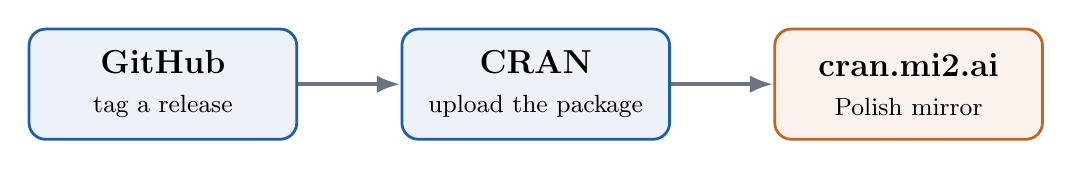
\begin{tikzpicture}[box/.style={draw=streamc,fill=streamc!8,rounded corners=6pt,line width=1pt,minimum width=3.4cm,minimum height=1.4cm,align=center,font=\large\bfseries},
                      arr/.style={-{Latex[length=3mm]},line width=1.6pt,color=greyc}]
    \node[box] (a) {GitHub\\{\normalfont\small tag a release}};
    \node[box,right=1.3cm of a] (b) {CRAN\\{\normalfont\small upload the package}};
    \node[box,right=1.3cm of b,draw=batchc,fill=batchc!8] (c) {cran.mi2.ai\\{\normalfont\small Polish mirror}};
    \draw[arr] (a) -- (b); \draw[arr] (b) -- (c);
  \end{tikzpicture}

  \vspace{1.2cm}
  {\Large Nobody sees what happens next, \textbf{in near real time}.}
\end{frame}

\begin{frame}{What we want to know}
  \centering\vspace{0.2cm}
  \card{3.6cm}{streamc}{Forecast load}{Hourly downloads, 7 days ahead}\hspace{0.2cm}
  \card{3.6cm}{badc}{Spot bots}{Bots and CI runners, from behaviour}\hspace{0.2cm}
  \card{3.6cm}{batchc}{Measure lag}{Release to download peak}

  \vspace{1.2cm}
  {\large\color{greyc} For the mirror operator (MI2.ai) and R package maintainers}
\end{frame}

% ===========================================================================
\section{2 \ Raw data}
% ===========================================================================
\begin{frame}{Three sources}
  \centering\vspace{0.2cm}
  \card{3.6cm}{streamc}{Access log}{Mirror web server\\text, a stream}\hspace{0.2cm}
  \card{3.6cm}{batchc}{GitHub events}{REST API\\JSON, polled}\hspace{0.2cm}
  \card{3.6cm}{greyc}{crantogit}{package $\to$ repo map\\CSV, daily}
\end{frame}

\begin{frame}[fragile]{CRAN access log}
  \vspace{0.3cm}
  {\fontsize{8}{10}\selectfont\ttfamily 23.21.250.48 - - [15/Oct/2026:14:06:45 +0000]\\
  "GET /src/contrib/Archive/DescTools/DescTools\_0.99.14.tar.gz\\
  HTTP/1.1" 200 2009727}

  \vspace{0.9cm}
  \begin{itemize}
    \item $\sim$2--4 requests per second
    \item No User-Agent in the log
    \item Much traffic from outside Poland
  \end{itemize}
\end{frame}

\begin{frame}{GitHub Events API}
  \begin{columns}[c]
    \begin{column}{0.4\textwidth}
      \centering\bignum{4cm}{batchc}{5\,000}\\[0.3ex]{\large requests per hour}
    \end{column}
    \begin{column}{0.58\textwidth}
      \begin{itemize}
        \item Two polling tiers
        \item ETags: an unchanged timeline costs nothing
        \item 2\,627 watch-list rows in our test run
      \end{itemize}
    \end{column}
  \end{columns}
\end{frame}

\begin{frame}{crantogit mapping}
  \begin{columns}[c]
    \begin{column}{0.4\textwidth}
      \centering\bignum{4cm}{streamc}{18\,000}\\[0.3ex]{\large R packages}
    \end{column}
    \begin{column}{0.58\textwidth}
      \begin{itemize}
        \item Package $\to$ GitHub repository
        \item Joins downloads with releases
        \item 10--15\% are not on GitHub
      \end{itemize}
    \end{column}
  \end{columns}
\end{frame}

% ===========================================================================
\section{3 \ Architecture}
% ===========================================================================
\begin{frame}{Lambda architecture}
  \centering
  \resizebox{\textwidth}{!}{%
  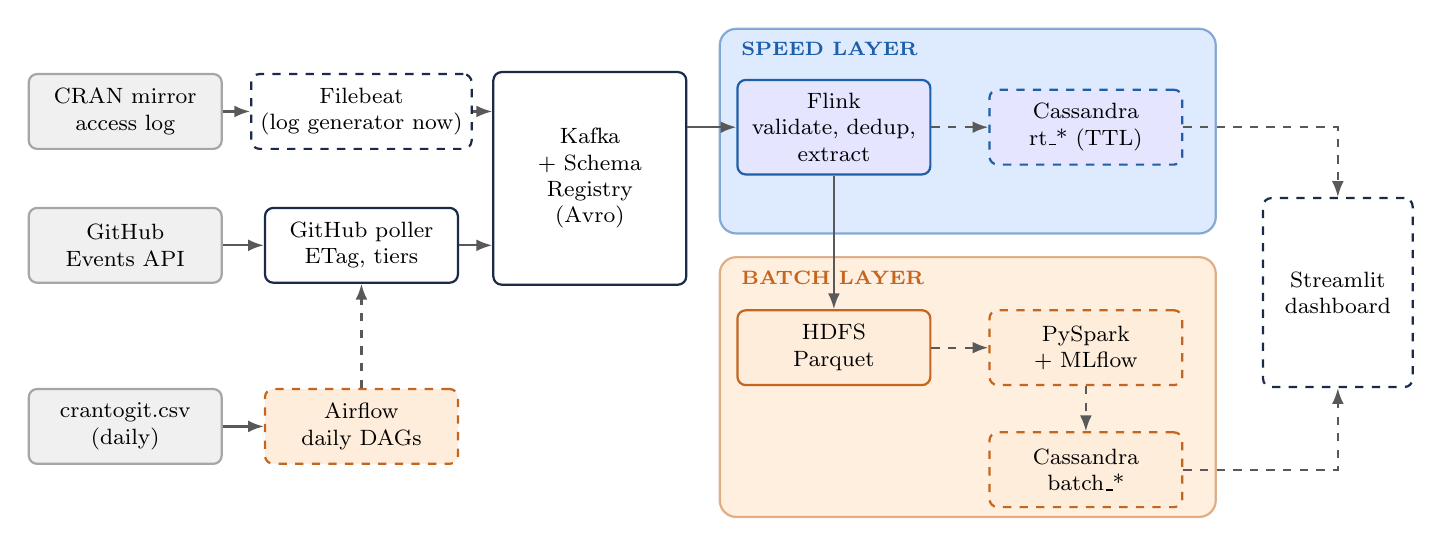
\begin{tikzpicture}[x=1cm,y=1cm,
    box/.style={draw,rounded corners=3pt,minimum width=2.45cm,minimum height=0.95cm,align=center,font=\footnotesize,thick},
    src/.style={box,fill=gray!12,draw=gray!70},
    stream/.style={box,fill=blue!10,draw=streamc},
    batch/.style={box,fill=orange!14,draw=batchc},
    shared/.style={box,fill=white,draw=navy},
    plan/.style={dashed},
    flow/.style={-{Latex[length=2mm]},thick,gray!70!black},
    pflow/.style={-{Latex[length=2mm]},thick,gray!70!black,dashed},
    lab/.style={font=\bfseries\scriptsize,anchor=north west}]
    \begin{scope}[on background layer]
      \fill[blue!60!cyan,opacity=0.13,rounded corners=6pt] (7.55,1.05) rectangle (13.85,-1.55);
      \draw[streamc,opacity=0.5,rounded corners=6pt,thick] (7.55,1.05) rectangle (13.85,-1.55);
      \fill[orange,opacity=0.13,rounded corners=6pt] (7.55,-1.85) rectangle (13.85,-5.15);
      \draw[batchc,opacity=0.5,rounded corners=6pt,thick] (7.55,-1.85) rectangle (13.85,-5.15);
    \end{scope}
    \node[lab,text=streamc] at (7.7,1.0) {SPEED LAYER};
    \node[lab,text=batchc] at (7.7,-1.9) {BATCH LAYER};
    \node[src] (logs) at (0,0.0) {CRAN mirror\\access log};
    \node[src] (gh) at (0,-1.7) {GitHub\\Events API};
    \node[src] (ctg) at (0,-4.0) {crantogit.csv\\(daily)};
    \node[shared,plan] (fb) at (3.0,0.0) {Filebeat\\(log generator now)};
    \node[shared] (poll) at (3.0,-1.7) {GitHub poller\\ETag, tiers};
    \node[batch,plan] (af) at (3.0,-4.0) {Airflow\\daily DAGs};
    \node[shared,minimum height=2.7cm] (kafka) at (5.9,-0.85) {Kafka\\+ Schema\\Registry\\(Avro)};
    \node[stream,minimum height=1.2cm] (flink) at (9.0,-0.2) {Flink\\validate, dedup,\\extract};
    \node[stream,plan] (rt) at (12.2,-0.2) {Cassandra\\rt\_* (TTL)};
    \node[batch] (hdfs) at (9.0,-3.0) {HDFS\\Parquet};
    \node[batch,plan] (spark) at (12.2,-3.0) {PySpark\\+ MLflow};
    \node[batch,plan] (bt) at (12.2,-4.55) {Cassandra\\batch\_*};
    \node[shared,plan,minimum height=2.4cm,minimum width=1.9cm] (st) at (15.4,-2.3) {Streamlit\\dashboard};
    \draw[flow] (logs) -- (fb); \draw[flow] (gh) -- (poll); \draw[flow] (ctg) -- (af);
    \draw[flow] (fb) -- (kafka.west |- fb); \draw[flow] (poll) -- (kafka.west |- poll);
    \draw[pflow] (af) -- (poll);
    \draw[flow] (kafka.east |- flink) -- (flink);
    \draw[flow] (flink.south) -- (hdfs.north);
    \draw[pflow] (flink) -- (rt);
    \draw[pflow] (hdfs) -- (spark);
    \draw[pflow] (spark) -- (bt);
    \draw[pflow] (rt.east) -| (st.north);
    \draw[pflow] (bt.east) -| (st.south);
  \end{tikzpicture}}

  \vspace{1ex}
  {\small\textcolor{greyc}{Dashed = work in progress}}
\end{frame}

\begin{frame}{One Kafka log, two layers}
  \begin{columns}[c]
    \begin{column}{0.48\textwidth}
      \card{5.2cm}{streamc}{Speed layer}{Flink: seconds of latency\\Cassandra with a TTL}
    \end{column}
    \begin{column}{0.48\textwidth}
      \card{5.2cm}{batchc}{Batch layer}{HDFS and Spark: full history\\forecasts and models}
    \end{column}
  \end{columns}
\end{frame}

\begin{frame}{Flink checks every record}
  \centering\vspace{0.2cm}
  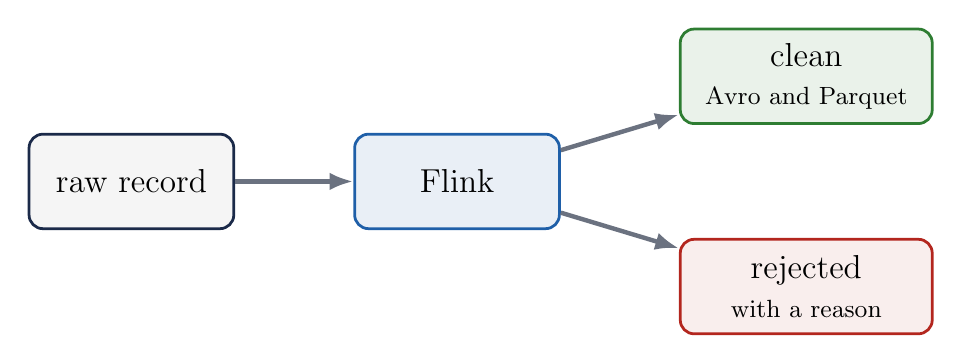
\begin{tikzpicture}[box/.style={draw,rounded corners=5pt,line width=1pt,minimum height=1.2cm,align=center,font=\large},
                      arr/.style={-{Latex[length=3mm]},line width=1.6pt,color=greyc}]
    \node[box,draw=navy,fill=gray!8,minimum width=2.6cm] (raw) {raw record};
    \node[box,draw=streamc,fill=streamc!10,right=1.5cm of raw,minimum width=2.6cm] (fl) {Flink};
    \node[box,draw=okc,fill=okc!10,above right=0.1cm and 1.5cm of fl,minimum width=3.2cm] (ok) {clean\\{\small Avro and Parquet}};
    \node[box,draw=badc,fill=badc!8,below right=0.1cm and 1.5cm of fl,minimum width=3.2cm] (bad) {rejected\\{\small with a reason}};
    \draw[arr] (raw) -- (fl); \draw[arr] (fl) -- (ok); \draw[arr] (fl) -- (bad);
  \end{tikzpicture}

  \vspace{0.9cm}
  {\Large The raw record is always kept unchanged.}
\end{frame}

\begin{frame}{How the topics fit together}
  \centering
  \resizebox{\textwidth}{!}{%
  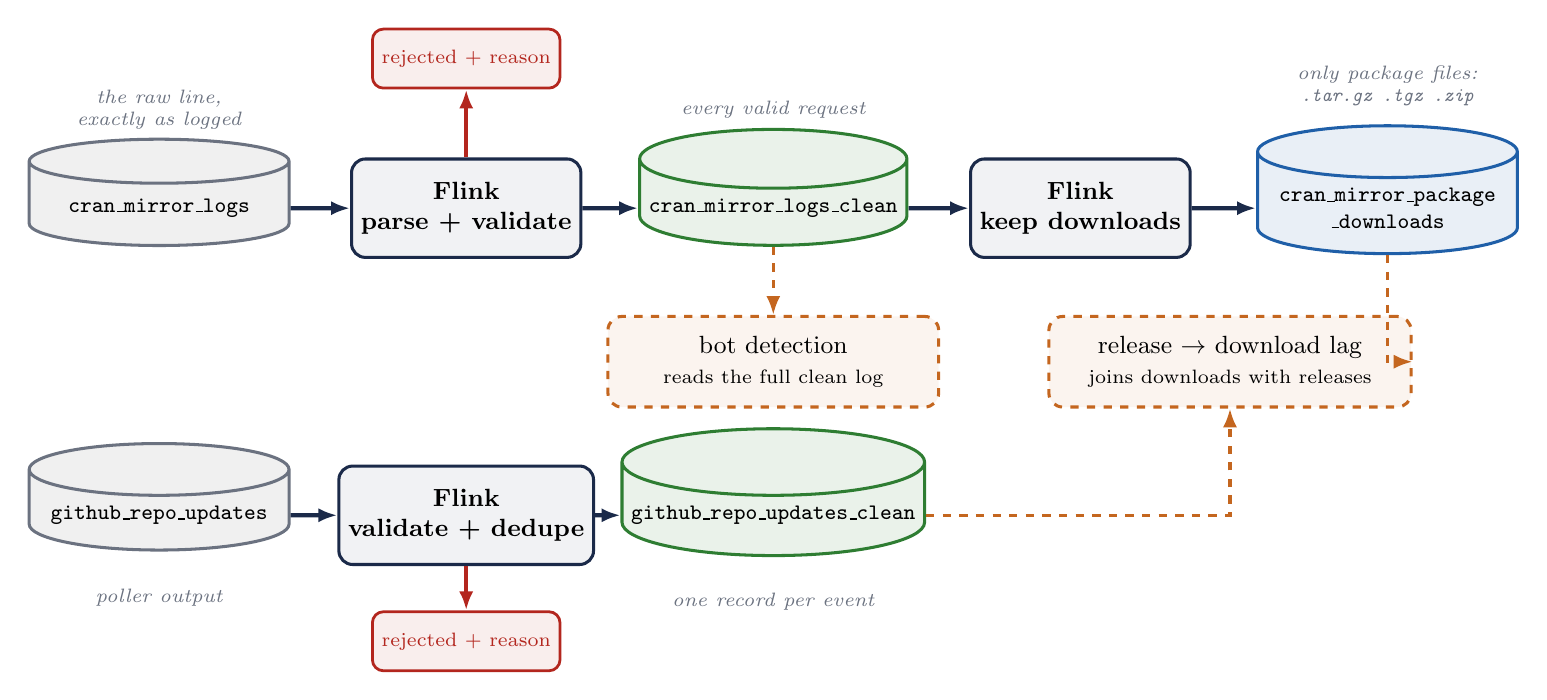
\begin{tikzpicture}[x=1cm,y=1cm,
    topic/.style={cylinder,shape border rotate=90,aspect=0.22,draw,line width=1.1pt,minimum height=1.35cm,minimum width=3.3cm,align=center,font=\footnotesize\ttfamily},
    rawt/.style={topic,draw=greyc,fill=gray!12},
    cleant/.style={topic,draw=okc,fill=okc!10},
    derivt/.style={topic,draw=streamc,fill=streamc!10},
    job/.style={draw=navy,fill=navy!6,rounded corners=5pt,line width=1.1pt,minimum height=1.25cm,minimum width=2.7cm,align=center,font=\small\bfseries},
    bad/.style={draw=badc,fill=badc!8,rounded corners=4pt,line width=1pt,minimum height=0.75cm,align=center,font=\scriptsize\color{badc}},
    use/.style={draw=batchc,dashed,fill=batchc!7,rounded corners=5pt,line width=1.1pt,align=center,font=\small},
    flow/.style={-{Latex[length=2.4mm]},line width=1.5pt,color=navy},
    uflow/.style={-{Latex[length=2.4mm]},line width=1.2pt,color=batchc,dashed},
    note/.style={font=\scriptsize\itshape,color=greyc,align=center}]
    % ---- CRAN lane
    \node[rawt] (raw) at (0,0) {cran\_mirror\_logs};
    \node[job] (j1) at (3.9,0) {Flink\\parse + validate};
    \node[cleant] (clean) at (7.8,0) {cran\_mirror\_logs\_clean};
    \node[job] (j2) at (11.7,0) {Flink\\keep downloads};
    \node[derivt] (dl) at (15.6,0) {cran\_mirror\_package\\\_downloads};
    \draw[flow] (raw) -- (j1); \draw[flow] (j1) -- (clean); \draw[flow] (clean) -- (j2); \draw[flow] (j2) -- (dl);
    \node[bad] (b1) at (3.9,1.9) {rejected + reason};
    \draw[flow,color=badc] (j1) -- (b1);
    \node[note] at (0,1.25) {the raw line,\\exactly as logged};
    \node[note] at (7.8,1.25) {every valid request};
    \node[note] at (15.6,1.55) {only package files:\\\texttt{.tar.gz .tgz .zip}};
    % ---- GitHub lane
    \node[rawt] (ghr) at (0,-3.9) {github\_repo\_updates};
    \node[job] (j3) at (3.9,-3.9) {Flink\\validate + dedupe};
    \node[cleant] (ghc) at (7.8,-3.9) {github\_repo\_updates\_clean};
    \draw[flow] (ghr) -- (j3); \draw[flow] (j3) -- (ghc);
    \node[bad] (b3) at (3.9,-5.5) {rejected + reason};
    \draw[flow,color=badc] (j3) -- (b3);
    \node[note] at (0,-4.95) {poller output};
    \node[note] at (7.8,-5.0) {one record per event};
    % ---- consumers (planned): each reads the topic it needs
    \node[use,minimum width=4.2cm,minimum height=1.15cm] (u1) at (7.8,-1.95) {bot detection\\{\scriptsize reads the full clean log}};
    \node[use,minimum width=4.6cm,minimum height=1.15cm] (u2) at (13.6,-1.95) {release $\to$ download lag\\{\scriptsize joins downloads with releases}};
    \draw[uflow] (clean) -- (u1);
    \draw[uflow] (dl.south) |- (u2.east);
    \draw[uflow] (ghc.east) -| (u2.south);
  \end{tikzpicture}}

  {\footnotesize \textcolor{greyc}{Every step writes to a topic, so anyone can read from any stage. Dashed = planned consumers.}}
\end{frame}

% ===========================================================================
\section{4 \ Our setup}
% ===========================================================================
\begin{frame}{Three environments}
  \centering\vspace{0.2cm}
  \card{3.6cm}{greyc}{Dev}{Laptop\\Docker volumes}\hspace{0.2cm}
  \card{3.6cm}{streamc}{Stage}{VM on the\\mirror's network}\hspace{0.2cm}
  \card{3.6cm}{batchc}{Prod}{Identical VM\\same network}
\end{frame}

\begin{frame}{Two identical VMs}
  \centering\vspace{0.3cm}
  \bignum{2.9cm}{streamc}{16}\bignum{2.9cm}{streamc}{64}\bignum{2.9cm}{streamc}{100}\bignum{2.9cm}{streamc}{1}\\[0.2ex]
  {\large\hspace{0.3cm}\makebox[2.9cm]{CPU cores}\makebox[2.9cm]{GB RAM}\makebox[2.9cm]{GB SSD}\makebox[2.9cm]{TB HDD}}

  \vspace{1.0cm}
  {\large On the \textbf{mirror's network}, static IPs, SSH through a bastion}
\end{frame}

\begin{frame}{One Compose file, four profiles}
  \centering\vspace{0.2cm}
  \Large
  \begin{tabular}{@{}ll@{}}
    \texttt{(none)} & core platform \\[0.6ex]
    \texttt{ha} & 3 DataNodes, replication 2 \\[0.6ex]
    \texttt{dev} & log generator \\[0.6ex]
    \texttt{github} & poller and its Flink job \\
  \end{tabular}

  \vspace{0.8cm}
  {\large Environments differ only in an env file}
\end{frame}

\begin{frame}[fragile]{Deploy with scripts}
  \vspace{0.3cm}
  {\fontsize{11}{15}\selectfont\ttfamily
  deploy/up.sh\\
  deploy/start\_logs.sh\\
  deploy/start\_github.sh\\
  deploy/inspect.sh}

  \vspace{0.8cm}
  {\large Idempotent: safe to run again}
\end{frame}

% ===========================================================================
\section{5 \ Tests}
% ===========================================================================
\begin{frame}{21 tests, all pass}
  \begin{columns}[c]
    \begin{column}{0.4\textwidth}
      \centering\bignum{4cm}{okc}{21/21}
    \end{column}
    \begin{column}{0.58\textwidth}
      \begin{itemize}
        \item 8 acquisition
        \item 6 pre-processing
        \item 7 quality
      \end{itemize}
    \end{column}
  \end{columns}

  \vspace{0.6cm}
  \centering{\large Fresh stack, live data plus marked test records}
\end{frame}

\begin{frame}{Bad data is rejected, with a reason}
  \centering\vspace{0.2cm}
  \large
  \begin{tabular}{@{}p{4.6cm}p{4.2cm}@{}}
    \toprule
    \textbf{Injected defect} & \textbf{Result} \\
    \midrule
    not a log line & \texttt{unparseable} \\
    status 999 & \texttt{invalid\_status} \\
    method FOO & \texttt{invalid\_method} \\
    date one day ahead & \texttt{future\_timestamp} \\
    date 30 days ago & \texttt{stale\_timestamp} \\
    \bottomrule
  \end{tabular}
\end{frame}

\begin{frame}{Nothing is lost}
  \centering\vspace{0.3cm}
  \bignum{3.2cm}{navy}{2462}\bignum{1.2cm}{greyc}{=}\bignum{3.2cm}{okc}{2456}\bignum{1.2cm}{greyc}{+}\bignum{2.0cm}{badc}{6}\\[0.2ex]
  {\large\hspace{0.1cm}\makebox[3.2cm]{raw lines}\makebox[1.2cm]{}\makebox[3.2cm]{clean}\makebox[1.2cm]{}\makebox[2.0cm]{rejected}}

  \vspace{1.0cm}
  {\large CRAN logs, read back from HDFS with pandas}
\end{frame}

\begin{frame}{A restarted poller does not repeat itself}
  \centering\vspace{0.3cm}
  \bignum{3.6cm}{streamc}{214}\bignum{3.6cm}{batchc}{9}\bignum{3.6cm}{okc}{0}\\[0.2ex]
  {\large\makebox[3.6cm]{polls after restart}\makebox[3.6cm]{answered 304}\makebox[3.6cm]{duplicates}}

  \vspace{1.0cm}
  {\large Stored ETags and event ids survive the restart}
\end{frame}

% ===========================================================================
\section{6 \ Future steps}
% ===========================================================================
\begin{frame}{Next: real data}
  \begin{itemize}
    \item Filebeat on the original mirror
    \item Real volumes on stage and prod
    \item GeoIP enrichment
  \end{itemize}
\end{frame}

\begin{frame}{Then: batch, models and dashboard}
  \begin{itemize}
    \item Airflow and Spark jobs
    \item Cassandra tables
    \item MLflow: load forecast, bot classifier
    \item Streamlit dashboard
  \end{itemize}
\end{frame}

\begin{frame}[plain]
  \centering
  \vspace{2.6cm}
  {\Huge\bfseries\color{navy} Thank you}\\[1.2ex]
  {\Large\color{greyc} Questions?}
\end{frame}

\end{document}
